%%%%%%%%%%%%%%%%%%%%%%%%%%%%%%%%%%%%%%%%%
% Beamer Presentation
% LaTeX Template
% Version 1.0 (10/11/12)
%
% This template has been downloaded from:
% http://www.LaTeXTemplates.com
%
% License:
% CC BY-NC-SA 3.0 (http://creativecommons.org/licenses/by-nc-sa/3.0/)
%
%%%%%%%%%%%%%%%%%%%%%%%%%%%%%%%%%%%%%%%%%

%----------------------------------------------------------------------------------------
%	PACKAGES AND THEMES
%----------------------------------------------------------------------------------------

\documentclass{beamer}

\mode<presentation> {

% The Beamer class comes with a number of default slide themes
% which change the colors and layouts of slides. Below this is a list
% of all the themes, uncomment each in turn to see what they look like.

%\usetheme{default}
%\usetheme{AnnArbor}
%\usetheme{Antibes}
%\usetheme{Bergen}
%\usetheme{Berkeley}
%\usetheme{Berlin}
%\usetheme{Boadilla}
%\usetheme{CambridgeUS}
%\usetheme{Copenhagen}
%\usetheme{Darmstadt}
%\usetheme{Dresden}
%\usetheme{Frankfurt}
%\usetheme{Goettingen}
%\usetheme{Hannover}
%\usetheme{Ilmenau}
%\usetheme{JuanLesPins}
%\usetheme{Luebeck}
\usetheme{Madrid}
%\usetheme{Malmoe}
%\usetheme{Marburg}
%\usetheme{Montpellier}
%\usetheme{PaloAlto}
%\usetheme{Pittsburgh}
%\usetheme{Rochester}
%\usetheme{Singapore}
%\usetheme{Szeged}
%\usetheme{Warsaw}

% As well as themes, the Beamer class has a number of color themes
% for any slide theme. Uncomment each of these in turn to see how it
% changes the colors of your current slide theme.

%\usecolortheme{albatross}
%\usecolortheme{beaver}
%\usecolortheme{beetle}
%\usecolortheme{crane}
%\usecolortheme{dolphin}
%\usecolortheme{dove}
%\usecolortheme{fly}
%\usecolortheme{lily}
%\usecolortheme{orchid}
%\usecolortheme{rose}
%\usecolortheme{seagull}
%\usecolortheme{seahorse}
%\usecolortheme{whale}
%\usecolortheme{wolverine}

%\setbeamertemplate{footline} % To remove the footer line in all slides uncomment this line
%\setbeamertemplate{footline}[page number] % To replace the footer line in all slides with a simple slide count uncomment this line

%\setbeamertemplate{navigation symbols}{} % To remove the navigation symbols from the bottom of all slides uncomment this line
}

\usepackage{graphicx} % Allows including images
\usepackage{booktabs} % Allows the use of \toprule, \midrule and \bottomrule in tables
\usepackage{cool}
\usepackage{tikz}
\usepackage{amsmath}
\usepackage{xcolor}
\usepackage{hyperref}

\DeclareMathOperator*{\argmax}{argmax}
\DeclareMathOperator*{\argmin}{argmin}
\usetikzlibrary{positioning}

%----------------------------------------------------------------------------------------
%	TITLE PAGE
%----------------------------------------------------------------------------------------

\title[RL for Finance]{CME 241: Reinforcement Learning for Stochastic Control Problems in Finance} % The short title appears at the bottom of every slide, the full title is only on the title page

\author{Ashwin Rao} % Your name
\institute[Stanford] % Your institution as it will appear on the bottom of every slide, may be shorthand to save space
{ICME, Stanford University
 % Your institution for the title page
}

\date{} % Date, can be changed to a custom date

\begin{document}
\begin{frame}
\titlepage % Print the title page as the first slide
\end{frame}

% \begin{frame}
% \frametitle{Overview} % Table of contents slide, comment this block out to remove it
% \tableofcontents % Throughout your presentation, if you choose to use \section{} and \subsection{} commands, these will automatically be printed on this slide as an overview of your presentation
% \end{frame}

\begin{frame}
\frametitle{Overview of the Course}
\begin{itemize}
\item Theory of Markov Decision Processes (MDPs)
\item Dynamic Programming (DP) Algorithms (a.k.a. model-based)
\item Reinforcement Learning (RL) Algorithms (a.k.a. model-free)
\item Plenty of Python implementations of models and algorithms
\item Apply these algorithms to 3 Financial/Trading problems:
\begin{itemize}
\item (Dynamic) Asset-Allocation to maximize utility of Consumption
\item Optimal Exercise/Stopping of Path-dependent American Options
\item Optimal Trade Order Execution (managing Price Impact)
\end{itemize}
\item By treating each of the problems as MDPs (i.e., Stochastic Control)
\item We will go over classical/analytical solutions to these problems
\item Then introduce real-world considerations, and tackle with RL (or DP)
\end{itemize}
\end{frame}

\begin{frame}
\frametitle{What is the flavor of this course?}
An important goal of this course is to effectively blend:
\begin{itemize}
\item Theory/Mathematics
\item Programming/Algorithms
\item Modeling of Read-World Finance/Trading Problems
\end{itemize}
\end{frame}


\begin{frame}
\frametitle{Pre-Requisites and Housekeeping}
\begin{itemize}
\item Theory Pre-reqs: Optimization, Probability, Pricing, Portfolio Theory
\item Coding Pre-reqs: Data Structures/Algorithms with numpy/scipy
\item Alternative: Written test to demonstrate above-listed background
\item Grade based on Class Participation, 2 Exams, and Programming Work
\item Passing grade fetches 3 credits, can be applied towards MCF degree
\item Wed and Fri 4:30pm - 5:50pm, 01/07/2019 - 03/15/2019
\item Classes in Building 160 (Wallenberg Hall) - Room 321
\item Appointments: Any time Fridays or an hour before class Wednesdays
\item Use appointments time to discuss theory as well as your code
\end{itemize}
\end{frame}

\begin{frame}
\frametitle{Resources}
\begin{itemize}
\item I recommend \href{http://incompleteideas.net/book/the-book-2nd.html}{\underline{\textcolor{blue}{Sutton-Barto}}} as the companion book for this course
\begin{itemize}
\item I won't follow the structure of Sutton-Barto book
\item But I will follow his approach/treatment
\end{itemize}
\item I will follow the structure of \href{http://www0.cs.ucl.ac.uk/staff/d.silver/web/Teaching.html}{\underline{\textcolor{blue}{David Silver's RL course}}}
\begin{itemize}
\item I encourage you to augment my lectures with David's lecture videos
\item Occasionally, I will wear away or speed up/slow down from this flow
\end{itemize}
\item We will do a bit more Theory \& a lot more coding (relative to above)
\item You can freely use my \href{https://github.com/coverdrive/MDP-DP-RL}{\underline{\textcolor{blue}{open-source code}}} for your coding work
\begin{itemize}
\item I expect you to duplicate the functionality of above code in this course
\end{itemize}
\item We will go over some classical papers on the Finance applications
\item To understand in-depth the analytical solutions in simple settings
\item I will augment the above content with many of my own slides
\item All of this will be organized on the course web site
\end{itemize}
\end{frame}


\begin{frame}
\frametitle{The MDP Framework (that RL is based on)}
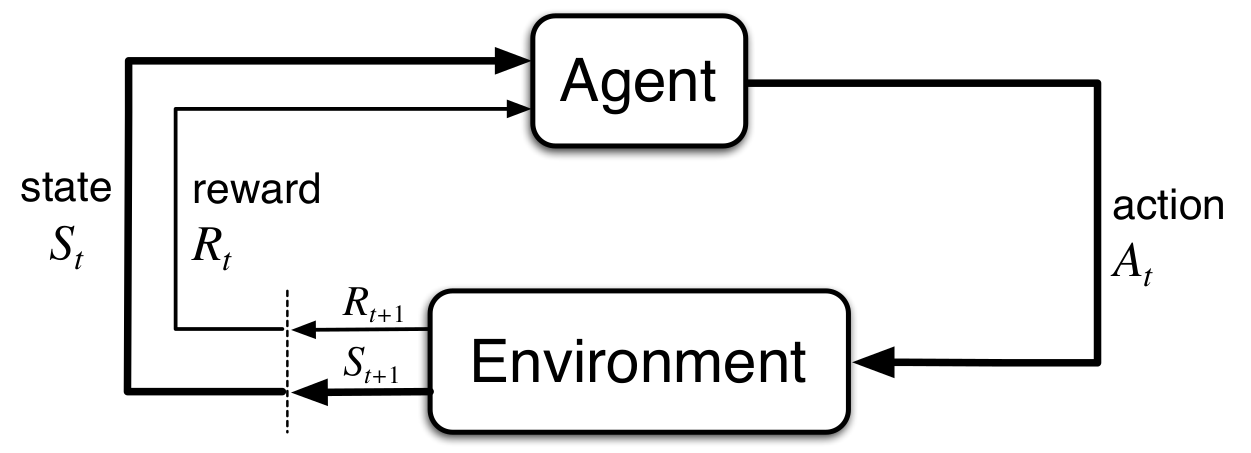
\includegraphics[width=12cm, height=7cm]{MDP.png}
\end{frame}

\begin{frame}
\frametitle{Components of the MDP Framework}
\begin{itemize}
\item The {\em Agent} and the {\em Environment} interact in a time-sequenced loop
\item {\em Agent} responds to [{\em State}, {\em Reward}] by taking an {\em Action}
\item {\em Environment} responds by producing next step's (random) {\em State}
\item {\em Environment} also produces a (random) scalar denoted as {\em Reward}
\item Goal of {\em Agent} is to maximize {\em Expected Sum} of all future {\em Reward}s
\item By controlling the ({\em Policy} : {\em State} $\rightarrow$ {\em Action}) function
\item {\em Agent} often doesn't know the {\em Model} of the {\em Environment}
\item {\em Model} refers to state-transition probabilities and reward function
\item So, {\em Agent} has to learn the {\em Model} AND learn the Optimal {\em Policy}
\item This is a dynamic (time-sequenced control) system under uncertainty
\end{itemize}
\end{frame}

\begin{frame}
\frametitle{Many real-world problems fit this MDP framework}
\begin{itemize}
\item Self-driving vehicle (speed/steering to optimize safety/time)
\item Game of Chess (Boolean {\em Reward} at end of game)
\item Complex Logistical Operations (eg: movements in a Warehouse)
\item Make a humanoid robot walk/run on difficult terrains
\item Manage an investment portfolio
\item Control a power station
\item Optimal decisions during a football game
\item Strategy to win an election (high-complexity MDP)
\end{itemize}
\end{frame}

\begin{frame}
\frametitle{Why are these problems hard?}
\begin{itemize}
\item {\em Model} of {\em Environment} is unknown (learn as you go)
\item {\em State} space can be large or complex (involving many variables)
\item Sometimes, {\em Action} space is also large or complex
\item No direct feedback on ``correct'' {\em Actions} (only feedback is {\em Reward})
\item {\em Action}s can have delayed consequences (late {\em Reward}s)
\item Time-sequenced complexity (eg: {\em Actions} influence future {\em Actions})
\item {\em Agent} {\em Action}s need to tradeoff between ``explore'' and ``exploit''
\end{itemize}
\end{frame}

\begin{frame}
\frametitle{Why is RL interesting/useful to learn about?}
\begin{itemize}
\item RL solves MDP problem when {\em Environment Model} is unknown
\item Also useful when {\em State} or {\em Action} space is too large/complex
\item {\bf Promise of modern A.I. is based on success of RL algorithms}
\item Potential for automated decision-making in real-world business
\item In 10 years: Bots that act or behave more optimal than humans
\item RL already solves various low-complexity real-world problems
\item RL will soon be the most-desired skill in the Data Science job-market
\item Possibilities in Finance are endless (we cover 3 important problems)
\item Learning RL is a lot of fun! (interesting in theory as well as coding)
\end{itemize}
\end{frame}

\begin{frame}
\frametitle{Optimal Asset Allocation to Maximize Consumption Utility}
\begin{itemize}
\item You can invest in (allocate wealth to) a collection of assets
\item Investment horizon is a fixed length of time
\item Each risky asset has an unknown distribution of returns
\item Transaction Costs \& Constraints on trading hours/quantities/shorting
\item Allowed to consume a fraction of your wealth at specific times
\item Dynamic Decision: Time-Sequenced Allocation \& Consumption
\item To maximize horizon-aggregated Utility of Consumption
\item Utility function represents degree of risk-aversion
\item So, we effectively maximize aggregate Risk-Adjusted Consumption
\end{itemize}
\end{frame}

\begin{frame}
\frametitle{MDP for Optimal Asset Allocation problem}
\begin{itemize}
\item {\em State} is [Current Time, Current Holdings, Current Prices]
\item {\em Action} is [Allocation Quantities, Consumption Quantity]
\item {\em Action}s limited by various real-world trading constraints
\item {\em Reward} is Utility of Consumption less Transaction Costs
\item {\em State}-transitions governed by risky asset movements
\end{itemize}
\end{frame}

\begin{frame}
\frametitle{Optimal Exercise of Path-Dependent American Options}
\begin{itemize}
\item RL is an alternative to Longstaff-Schwartz algorithm for Pricing
\item {\em State} is [Current Time, History of Underlying Security Prices]
\item {\em Action} is Boolean: Exercise (i.e., Payoff and Stop) or Continue
\item {\em Reward} always 0, except upon Exercise ($=$ Payoff)
\item {\em State}-transitions governed by Underlying Price's Stochastic Process
\item Optimal Policy $\Rightarrow$ Optimal Stopping $\Rightarrow$ Option Price
\item Can be generalized to other Optimal Stopping problems
\end{itemize}
\end{frame}

\begin{frame}
\frametitle{Optimal Trade Order Execution (controlling Price Impact)}
\begin{itemize}
\item You are tasked with selling a large qty of a (relatively less-liquid) stock
\item You have a fixed horizon over which to complete the sale
\item Goal is to maximize aggregate sales proceeds over horizon
\item If you sell too fast, {\em Price Impact} will result in poor sales proceeds
\item If you sell too slow, you risk running out of time
\item We need to model temporary and permanent {\em Price Impact}s
\item Objective should incorporate penalty for variance of sales proceeds
\item Which is equivalent to maximizing aggregate Utility of sales proceeds 
\end{itemize}
\end{frame}

\begin{frame}
\frametitle{MDP for Optimal Trade Order Execution}
\begin{itemize}
\item {\em State} is [Time Remaining, Stock Remaining to be Sold, Market Info]
\item {\em Action} is Quantity of Stock to Sell at current time
\item {\em Reward} is Utility of Sales Proceeds (i.e., Variance-adjusted-Proceeds)
\item {\em Reward} \& {\em State}-transitions governed by {\em Price Impact Model}
\item Real-world {\em Model} can be quite complex (Order Book Dynamics)
\end{itemize}
\end{frame}


\begin{frame}
\frametitle{Week by Week (Tentative) Schedule}
\begin{itemize}
\item W1: Markov Decision Processes \& Overview of Finance Problems
\item W2: Bellman Equations \& Dynamic Programming Algorithms
\item W3: Optimal Asset Allocation problem
\item W4: Optimal Exercise of American Options problem
\item W5: Optimal Trade Order Execution problem, and Mid-Term Exam
\item W6: Model-free Prediction (RL for Value Function Estimation)
\item W7: Model-Free Control (RL for Optimal Value Function/Policy)
\item W8: RL with Function Approximation (including Deep RL)
\item W9: Batch Methods (DQN, LSTDQ/LSPI), and Gradient TD
\item W10: Policy Gradient Algorithms, and Final Exam

\end{itemize}
\end{frame}

\begin{frame}
\frametitle{Sneak Peek into a few lectures in this course}
\begin{itemize}
\item \href{https://github.com/coverdrive/technical-documents/blob/master/finance/cme241/MertonPortfolio.pdf}{\underline{\textcolor{blue}{HJB Equation and Merton's Portfolio Problem}}}
\item \href{https://github.com/coverdrive/technical-documents/blob/master/finance/cme241/PolicyGradient.pdf}{\underline{\textcolor{blue}{Policy Gradient Theorem and Compatible Approximation Theorem}}}
\item \href{https://github.com/coverdrive/technical-documents/blob/master/finance/cme241/ValueFunctionGeometry.pdf}{\underline{\textcolor{blue}{Value Function Geometry and Gradient TD}}}
\end{itemize}
\end{frame}

\begin{frame}
\frametitle{Landmark Papers we will cover in detail}
\begin{itemize}
\item \href{https://www.jstor.org/stable/1926560}{\underline{\textcolor{blue}{Merton's solution for Optimal Portfolio Allocation/Consumption}}}
\item \href{https://people.math.ethz.ch/~hjfurrer/teaching/LongstaffSchwartzAmericanOptionsLeastSquareMonteCarlo.pdf}{\underline{\textcolor{blue}{Longstaff-Schwartz Algorithm for Pricing American Options}}}
\item \href{http://alo.mit.edu/wp-content/uploads/2015/06/Optimal-Control-of-Execution-Costs.pdf}{\underline{\textcolor{blue}{Bertsimas-Lo paper on Optimal Execution Cost}}}
\item \href{https://pdfs.semanticscholar.org/3d2d/773983c5201b58586af463f045befae5bbf2.pdf}{\underline{\textcolor{blue}{Almgren-Chriss paper on Optimal Risk-Adjusted Execution Cost}}}
\item \href{https://www.cs.toronto.edu/~vmnih/docs/dqn.pdf}{\underline{\textcolor{blue}{Original DQN paper}}} and \href{https://storage.googleapis.com/deepmind-media/dqn/DQNNaturePaper.pdf}{\underline{\textcolor{blue}{Nature DQN paper}}}
\item \href{http://www.jmlr.org/papers/volume4/lagoudakis03a/lagoudakis03a.pdf}{\underline{\textcolor{blue}{Lagoudakis-Parr paper on Least Squares Policy Iteration}}}
\item \href{http://papers.nips.cc/paper/1713-policy-gradient-methods-for-reinforcement-learning-with-function-approximation.pdf}{\underline{\textcolor{blue}{Sutton et al's paper on Policy Gradient}}}
\end{itemize}
\end{frame}


\begin{frame}
\frametitle{Similar Courses offered at Stanford}
\begin{itemize}
\item AA 228/CS 238 (Mykel Kochenderfer - Autumn 2018)
\item CS 234 (Emma Brunskill - Winter 2019)
\item MS\&E 251 (Edison Tse - Spring 2019)
\item CS 332 (Emma Brunskill - Autumn 2018)
\item MS\&E 338 (Ben Van Roy - Spring 2019)
\item MS\&E 348 (Gerd Infanger - Winter 2020)
\item MS\&E 351 (Ben Van Roy - Winter 2019)

\end{itemize}
\end{frame}

\end{document}